\documentclass{IEEEtran}
\usepackage[utf8]{inputenc}
\usepackage{graphicx}
\usepackage{hyperref}
\usepackage{xurl}
\usepackage{float}
\usepackage{tabularx}
\graphicspath{{./images/}}


% correct bad hyphenation here
\hyphenation{op-tical net-works semi-conduc-tor}


\title{Propuesta de arquitectura de control de versiones en bases de datos evolutivas.}

\author{\IEEEauthorblockN{ Gerardo Adolfo Salas Montoya}
\IEEEauthorblockA{\\Maestría en ingeniería de software con énfasis en arquitectura y diseño de software.\\
Universidad Cenfotec\\
San Jose, Costa Rica\\
Email: gsalasm@ucenfotec.ac.cr }}


\date{\today}



\begin{document}

\maketitle

\begin{abstract}
    Este artículo de maestría se centra en el estudio y la mejora de los procesos de control de versiones para bases de datos evolutivas, un área que ha recibido relativamente poca atención en la disciplina de ingeniería de software, sin embargo, es una práctica cada vez más demandada en los grupos de desarrollo. Las bases de datos están diseñadas para adaptarse y cambiar con el tiempo sin embargo el no tener un registro completo de los cambios que se aplican sobre cada uno de los objetos que la componen pueden llegar a causar diferentes problemas en los grupos de desarrollo y por su puesto en las bases de datos.
\end{abstract}
    
\begin{IEEEkeywords}
    Control de versiones de bases de datos,
    Bases de datos evolutivas,
    Integración/Despliegue continuo (CI/CD),
    Gestión de cambios en bases de datos,
    Arquitectura de bases de datos,
    Liquibase,
    Flyway,
    Automatización de despliegues,
    Mantenimiento de bases de datos,
    Desarrollo ágil de software
\end{IEEEkeywords}

\section{Introducción}
En el desarrollo de software moderno, las bases de datos desempeñan un rol fundamental para asegurar la adaptabilidad y flexibilidad de las aplicaciones. El concepto de bases de datos evolutivas surge como respuesta a la necesidad de las organizaciones de adaptarse rápidamente a cambios en los requisitos y necesidades del negocio, integrándose efectivamente en los procesos de Integración Continua y Despliegue Continuo (CI/CD). Sin embargo, la gestión de versiones en este tipo de bases de datos plantea desafíos significativos, ya que las herramientas tradicionales de control de versiones no están diseñadas para manejar la complejidad y estructura de las bases de datos, lo cual con frecuencia resulta en inconsistencias y problemas de implementación.

Este proyecto aborda la problemática de la falta de una arquitectura robusta de control de versiones para bases de datos evolutivas, lo cual afecta la calidad y eficiencia de los procesos de CI/CD en las organizaciones. La propuesta tiene como objetivo desarrollar una arquitectura de control de versiones específica para bases de datos que evolucionan constantemente, buscando reducir riesgos de errores y conflictos en los cambios, mejorar la consistencia de los datos y facilitar la integración rápida y frecuente de nuevas características. Además, esta solución permitirá mantener un registro exhaustivo de todos los cambios, apoyando tanto la implementación de mejoras como la corrección de errores.

Desde el punto de vista técnico, herramientas como Liquibase y Flyway ofrecen funcionalidades clave que pueden adaptarse y optimizarse para satisfacer las necesidades de control de versiones en bases de datos.
Operativamente, el proyecto es viable, ya que muchas organizaciones ya emplean prácticas de control de versiones en sus procesos de CI/CD, y la integración de una arquitectura específica para bases de datos no requerirá cambios disruptivos, sino mejoras y adaptaciones efectivas.

Conforme al paradigma Objetivo-Pregunta-Métrica (GQM) \cite{Basili1992}, el objetivo de esta investigación se puede enunciar de la siguiente manera:

\begin{itemize}
    \item[] {\textbf{\textit{Aplicar:}}} Una arquitectura para el control de versiones en bases de datos que cambian con frecuencia.
    \item[] {\textbf{\textit{Con el propósito de:}}} mejorar la trazabilidad, consistencia y facilidad de integración de los cambios en la base de datos en entornos de CI/CD.
    \item[] {\textbf{\textit{Con respecto a:}}} los desafíos en el rastreo y gestión de cambios en bases de datos.
    \item[] {\textbf{\textit{Desde el punto de vista de:}}} investigadores y profesionales de ingeniería de software enfocados en control de versiones y prácticas de CI/CD.
    \item[] {\textbf{\textit{En el contexto de:}}} mejorar las prácticas de control de versiones en organizaciones que dependen de actualizaciones frecuentes de bases de datos como parte de sus flujos de trabajo.
\end{itemize}


\vspace{0.5cm}
La estructura del resto del artículo es la siguiente. La Sección II presenta las preguntas de investigación. La Sección III discute los trabajos relacionados y el estado del arte. Los antecedentes se describen en la Sección IV. La metodología de investigación se explica en la Sección V, y los objetivos se presentan en las Secciones VI y VII. La Sección VIII describe las herramientas utilizadas para esta propuesta, "Liquibase" y "Flyway". La Sección IX aborda la descripción de la arquitectura propuesta para el control de cambios en bases de datos. La Sección X describe las pautas de la solucion. Finalmente, las Secciones XI y XII discuten los resultados, conclusiones y presentan el trabajo futuro.


\section{Preguntas de Investigación.}
This section lists the main research questions that we set out to answer.
\begin{itemize}
    \item Is the Moodle platform of University Cenfotec meeting the principles of accessibility outlined in WCAG 2.2?
    \item How can we improve the web accessibility of Universidad Cenfotec's Moodle by incorporating the main needs identified by the WCAG 2.2 guidelines to promote greater inclusion in the web ecosystem of Universidad Cenfotec?
\end{itemize}


\section{Related Work}
The following research has been conducted focusing on web accessibility within the context of e-learning software architecture:

In 2018, \cite{Schiavone2018} published an article titled "An analysis through experiences in scientific literature and a case study," where the focus is on analyzing the accessibility of the Moodle online learning platform, reviewing previous studies and evaluating the accessibility of specific Moodle installations.

\cite{Acosta2016} in 2016 conducted a comparative study of three Learning Management Systems (LMS), Moodle, Sakai, and the system called ABC, developed in Ecuador to evaluate the levels of accessibility according to users' needs. They analyzed and compared the selected LMSs based on accessibility criteria, considering functional tasks on a scale with 6 levels of accessibility that can be used for decision-making and LMS selection from the perspective of teachers and students.

\cite{Bocevska2018} published the research "Analysis of Accessibility of the e-Learning Platforms According to the WCAG 2.0 Standard Compliance," which aims to analyze the accessibility of the latest public versions of several Learning Management Systems (LMS), such as Moodle, Eliademy, Docebo, Sakai, and ATutor, for people with disabilities. The analysis will evaluate compliance with different levels of criteria established in the Web Content Accessibility Guidelines (WCAG).

The web accessibility project of the University of Costa Rica focuses on the application of international web accessibility standards, specifically on the WCAG 2.1 standard. Throughout the document, there is a reference to the importance of complying with these standards to ensure that websites are accessible to all users, including people with disabilities \cite{DaSilva}.

We also find the publication "AccGuideLiner: Towards a Modelling Approach of Web Accessibility Requirements following WCAG 2.2," which describes a detailed model for describing accessibility requirements by integrating expert knowledge and domain knowledge to simplify its implementation in tools. The document is aimed at web developers, designers, accessibility engineers, and researchers who wish to understand the guidelines and accessible requirements from the technical perspective to the code phase.

The main source of information is the guidelines established by WCAG 2.2 developed by the World Wide Web Consortium (W3C), which set technical standards and guidelines for creating more accessible web content for a wide range of users, including those with disabilities. These guidelines address key aspects such as perception, operability, and understanding of web content, ensuring it is accessible for both assistive technologies and users without disabilities.



\section{Background}
Many authors consider LMSs and their accessibility from different points of view. When the accessibility in context of e-learning is considered, many authors highlighted that there is a need to define criteria for instructors, authors of the contents and e-learning specialist that create and run activities on the web (Bocevska et al,2018).

Given that this research is conducted within the legal context of Costa Rica, we will adopt the definition of accessibility provided in Directive 051-MTSS-MICITT (Costa Rican Executive Branch, 2019). This directive defines accessibility as "the measures adopted by public and private institutions to ensure that persons with disabilities have access, on equal terms with others, to the physical environment, transportation, information and communications, including information and communication technologies and systems, and to other services and facilities open to the public or for public use. These measures also include the identification and removal of such barriers."

\section{Research Methodology}
The research method employed in the proposal involves several key steps. Initially, the chosen topic is clearly defined, followed by an extensive search for relevant literature addressing the research problem. Databases such as Google Scholar, EBSCO, and ResearchGate are utilized for this purpose  \cite{TTawalbeh2017}. Additionally, web searches are conducted to gather information on learning management systems (LMS), WCAG compliance, and tools available for evaluating web accessibility. During this process, detailed notes are taken to capture essential insights related to the research problem, and specific evaluation tools are selected. Citations are diligently recorded to facilitate the compilation of the references list later on. The gathered information is then analyzed and integrated into the project proposal, with key findings being summarized and thoroughly discussed this process follow Biolchini Technique.\cite{FerrariFabianoJose}.

Furthermore, accessibility testing and evaluation are performed on the latest public version of relevant LMS platforms, such as Moodle. The data collection process involves utilizing the IBM Equal Accessibility Checker plugin, which is installed in Google Chrome, to ensure comprehensive evaluation of web accessibility standards.
This methodical approach ensures that the research is thorough and systematic, laying a solid foundation for the project proposal and its objectives.


\section{Objective}
The main objective of this study is to evaluate the accessibility components of the Moodle e-learning platform and provide improvement recommendations based on the application of WCAG guidelines (version 2.2).

\section{Specific Objectives}
\begin{enumerate}
    \item Analyze the current accessibility components of the Moodle platform at Universidad Cenfotec using tools developed as plugins to analyze the entire accessibility infrastructure of a specific URL.
    \item Compare the principles and accessibility criteria established in WCAG 2.2 to determine their relevance and effectiveness for improving Moodle's accessibility.
    \item Develop recommendations based on the conducted research to address the most critical accessibility issues of Moodle at Universidad Cenfotec.
\end{enumerate}

\section{IBM equal accessibility checker}
To collect the WCAG 2.2 ratings on the analyzed pages, we used the "IBM Equal Accessibility Checker 7.3," which is an open-source tool (https://github.com/IBMa/equal-access) and available for free. It integrates into the browser's development tools and provides a comprehensive analysis environment through the auditor's or developer's browser, allowing for automatic accessibility evaluation of the visited page.This study is conducted using Google Chrome, and therefore, the tool is obtained through the official Google Chrome extension store.\cite{IBMAccessibilityEqualAccessToolkit}

We will use version 7.3, which includes six new success criteria from the Web Content Accessibility Guidelines (WCAG) 2.2 Level A and AA, as well as criteria that were already included in previous versions.

The rule set applied in this tool is grouped as follows:

\begin{itemize}
    \item Non-text content
    \item Keyboard content
    \item Language Parsing
\end{itemize}

The technique used for analysis relies on the tool's functionality, which checks various aspects of web accessibility in accordance with WCAG 2.2 guidelines, as mentioned earlier. It scans the pages to be analyzed, pinpointing potential accessibility issues and offering insights into elements that don't meet specified standards, such as exporting results in Excel format, among other functionalities.

Key features to note include:

\begin{itemize}
    \item Automatic scanning: The tool automatically analyzes the webpage, identifying areas of concern regarding accessibility.
    \item Comprehensive reports: Following the analysis, we thoroughly examine the detailed reports provided by the tool to draw conclusions and formulate recommendations aimed at improving accessibility.
\end{itemize}

This tools offers integrated accessibility testing through plug-ins and modules for Node JS and Karma \cite{Karma}
The URL that will be covered in the scope of the investigation are in the taxonomy of the page in next image

\begin{figure}[H]
    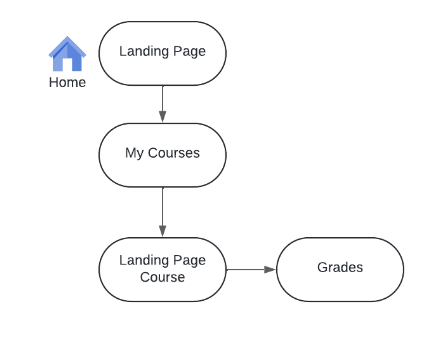
\includegraphics[width=0.48\textwidth]{images/figure1.png}
    \caption{Moodle page taxonomy}
    \label{fig:figure1}
\end{figure}

\section{MOODLE}
Moodle is one of the most popular open source LMS options available today. It features dashboards, learner tracking, and multimedia support. This open source Learning Management System also gives the ability to create mobile-friendly online courses integrating third party add-ons. One of the standouts of this tool is the user community \cite{Moodle2024}.

E-Learning has a series of conditions to have a successful learning process. The student's motivation and his/her level of responsibility and autonomy are crucial to achieve it. It is also important the quality of the digital materials and their design, as well as the appropriate learning situations and methodologies provided by the teacher to carry out learning, an accurate, quick and efficient tutoring are also fundamental elements \cite{Rahman2019}.

\section{WCAG}
The Web Content Accessibility Guidelines 2.2 \cite{W3C2023} was issued by the world's leading organization - The World Wide Web Consortium (W3C) on October 5, 2023.  In the following image are the differences between the tree version.

\begin{figure}[H]
    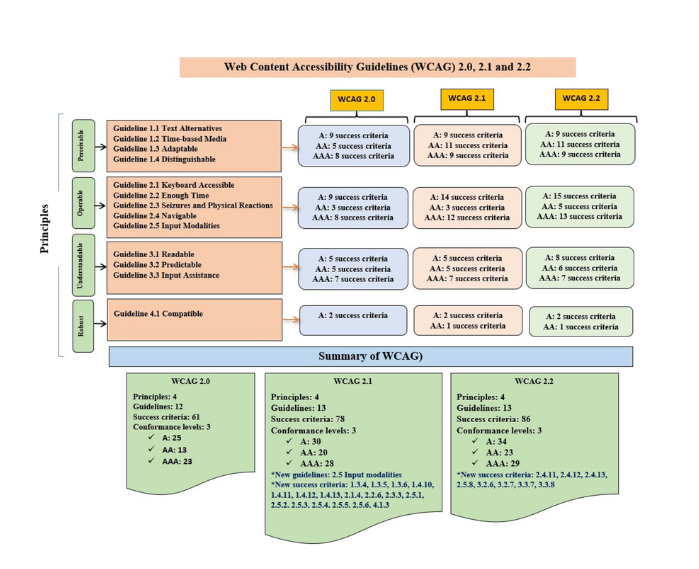
\includegraphics[width=0.48\textwidth]{images/figure2.png}
    \caption{ Web Content Accessibility Guidelines 2.0 / 2.1 / 2.2}
    \label{fig:figure2}
\end{figure}

Accessibility, usability, and inclusion are three important factors to be considered while developing a website usable by people with disabilities \cite{W3C2020}. The  WAI suggests a set of WCAG guidelines to be followed by developers of any website. Thus, each tool is checked if it follows at least one version of WCAG standards like WCAG 2.0, WCAG 2.1 and WCAG 2.2. 

Success criteria WCAG guidelines available at the W3C have a testable success criterion \cite{W3C2008} that can be categorized into three levels of conformance namely A, AA and AAA respectively. Each conformance level creates a better user experience for a wider audience. Thus, we ensured to select tools that follow at least two levels of conformance to evaluate a webpage no less than sufficiently accessible. The conformance levels are as follows:
\begin{itemize}
    \item Level A (Lowest Level): This holds the lowest level of accessibility success criterion to be satisfied by any website to be classified as accessible. A few suggestions by this level include-provide text alternatives for all non-text content; provide equivalent information for time-based media; create content that may be presented in multiple ways; use of color; audio and keyboard controls. 
    \item Level AA (Sufficient Level): This holds a higher level of accessibility success criterion than Level A. The website should meet all conditions mentioned in Level A. Additionally, it should include live audio caption; audio description; text contrast and resizing; text over images; appropriate labels/headings.
    \item Level AAA (Highest Level): This holds the highest level of accessibility success criterion. The website should successfully meet all the criteria mentioned in Level A and Level AA along with extended audio descriptions; sign languages; multimedia alternatives and interruptions; and content size.
\end{itemize} 

\subsection{POUR factors}
Guidelines and success criteria defined by the W3C are organized around four principles called the POUR factors. These principles lay the foundation necessary for anyone to access and use Web content with ease \cite{Moorman1999}. POUR is the abbreviation of Perceivable, Operable, Understandable and Robust. Each of the web accessibility evaluation tool is checked to follow at least one of the four factors. Additionally, information available on the website should be:


\begin{itemize}
    \item Perceivable: The user interface components and information on website must be presented in a way that can be perceived by users with ease.
    \item Operable: Navigation and user interface components must be operable. This is necessary for users to operate all components required for interaction.
    \item Understandable: Operation and information of the interface must be understandable by the user. This is necessary as users must be able to understand the information and operations offered by website.
    \item Robust: Contents of website should work across.
\end{itemize}



\section{Results}
The W3 Consortium provides a publicly available quick reference for objectively rating the integration of accessibility into a platform. The WCAG 2.2 guidelines have a list of categories that can be rated on three levels: A, AA, and AAA. The lowest category, A, indicates poor accessibility, while the AA category signifies meeting all criteria of the A rating plus additional criteria. The highest category, AAA, implies that the previous levels are met.

We have established different levels to categorize the issue founded in the analysis.

As we can see int the \ref{fig:figure3} it displays the issues and non-issues found in different sections of the Moodle platform that Universidad CENFOTEC uses for virtual education. The pages evaluated in this analysis are shown on the y-axis. It is worth noting that the "Landing Page" has a higher proportion of non-issues compared to issues, while the "Landing Page Course" has slightly more issues than non-issues. This graph can be used as a diagnostic tool to identify areas where web accessibility can be improved to comply with WCAG standards, ensuring an inclusive experience for all users.

\begin{figure}[H]
    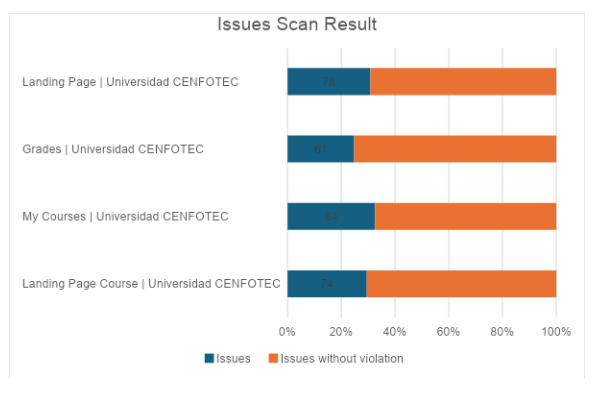
\includegraphics[width=0.48\textwidth]{images/scanResult.png}
    \caption{Issues scan result}
    \label{fig:figure3}
\end{figure}


Also, in the figure \ref{fig:figure4}, \ref{fig:figure5}, \ref{fig:figure6} and \ref{fig:figure7} the bar charts presents a comparison of web accessibility across different sections of the Moodle platform. The chart is devised to showcase compliance with WCAG standards focusing on the operability of web pages. The blue and orange bars facilitate an immediate visual comparison, with orange bars representing issues without a violation consistently outperforming the blue ones that represent violations to the WCAG principles. This suggests that the page has good accessibility. The evaluated categories include “Landing Page”, “My Courses”, “Grades”, and “Landing Page Course”. The highest bar reaches nearly the value of 35 on the Y-axis, indicating a high level of operable accessibility. Another way to interpret this chart is as an accessibility blueprint, where each bar represents a pillar of the web structure. The height of the bars reflects the solidity and compliance with accessibility principles, which is essential for building an inclusive web environment.
\begin{figure}[H]
    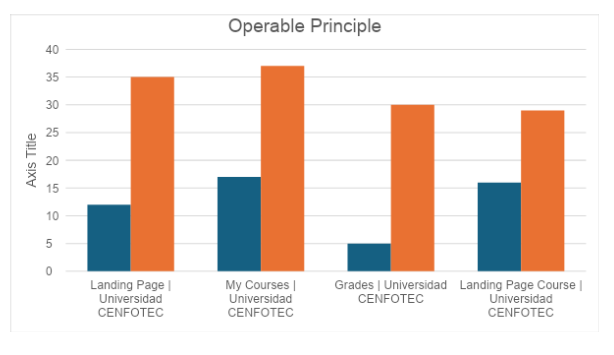
\includegraphics[width=0.48\textwidth]{images/operablePrinciple.png}
    \caption{Operable Principle}
    \label{fig:figure4}
\end{figure}
q
\begin{figure}[H]
    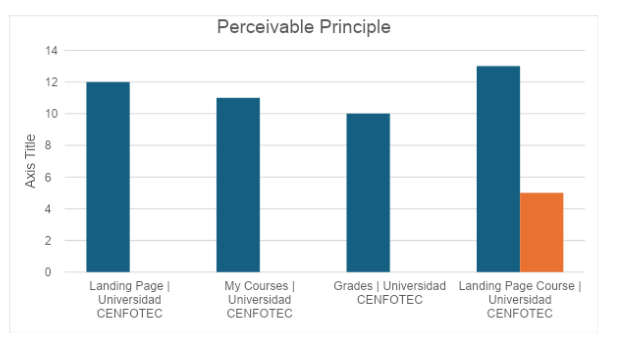
\includegraphics[width=0.48\textwidth]{images/perceivablePrinciple.png}
    \caption{Perceivable Principle}
    \label{fig:figure5}
\end{figure}
q
\begin{figure}[H]
    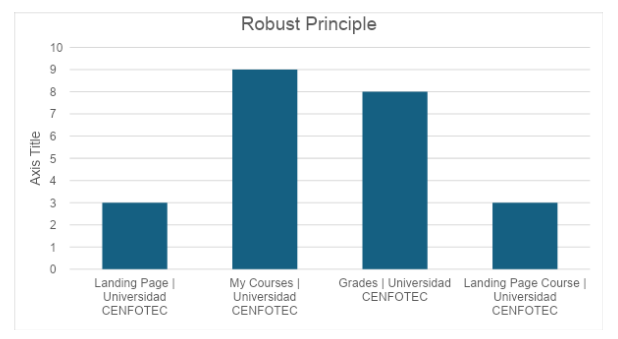
\includegraphics[width=0.48\textwidth]{images/robustPrinciple.png}
    \caption{Robust Principle}
    \label{fig:figure6}
\end{figure}
q
\begin{figure}[H]
    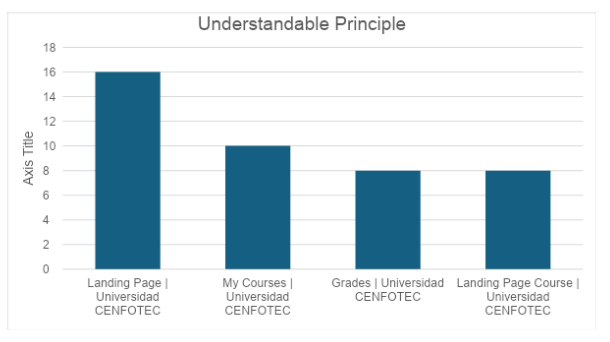
\includegraphics[width=0.48\textwidth]{images/undestandablePrinciple.png}
    \caption{Understandable Principle}
    \label{fig:figure7}
\end{figure}


The following is a comprehensive evaluation of the Moodle platform used by Universidad CENFOTEC, as summarized in \ref{tab:table1}. The evaluation highlights the acceptance criteria that have scored the highest and lowest across all sections of the platform. The criterion "3.2.2 On Input" has received the highest score of 16 for the "Landing Page", indicating that the platform has exceptional performance in handling user input. However, the criterion "1.4.1 Use of Color" has scored the lowest, suggesting potential improvements in color usage for a better user experience. Some criteria like "2.4.3 Focus Order" and "3.3.2 Labels or Instructions" have not received any scores, which may imply that they are either not applicable or have not been evaluated. By the same token, the "My Course" section has achieved the highest total score of 47, indicating that it has effectively complied with most acceptance criteria. Conversely, the "Grades" section, with the lowest total score of 31, might have more room for improvement. While these insights provide a quantitative overview of the platform's performance, they should be complemented with qualitative user feedback for a holistic understanding of the platform's functionality and user experience.

\vspace{2cm}
\begin{table}[h]
    \centering
    \caption{Acceptance Criteria (A)}
    \label{tab:table1}
    \begin{tabularx}{\columnwidth}{|l|X|X|X|X|}
    \hline
    \textbf{Acceptance Criteria} & \textbf{Grades} & \textbf{Landing Page} & \textbf{Landing Page Course} & \textbf{My Course} \\ 
    \hline
    1.1.1 Non-text Content & 2 & 4 & 5 & 5 \\ 
    \hline
    1.3.1 Info and Relationships & 7 & 7 & 7 & 5 \\
    \hline
    1.4.1 Use of Color & 1 & 1 & 1 & 1 \\
    \hline
    2.1.1 Keyboard & 1 & - & 6 & 2 \\
    \hline
    2.4.1 Bypass Blocks & 3 & 11 & 7 & 9 \\
    \hline
    2.4.3 Focus Order & - & - & - & 2 \\
    \hline
    2.5.3 Label in Name & 1 & 1 & 3 & 4 \\
    \hline
    3.2.2 On Input & 8 & 16 & 8 & 8 \\
    \hline
    3.3.2 Labels or Instructions & - & - & - & 2 \\
    \hline
    4.1.2 Name, Role, Value & 8 & 3 & 3 & 9 \\
    \hline
    \textbf{Total} & 31 & 43 & 40 & 47 \\
    \hline
    \end{tabularx}
\end{table}

\vspace{1cm}

The "Acceptance Criteria (AA)" represented in the \ref{tab:table2} shows a comprehensive evaluation of the Moodle platform utilized by Universidad CENFOTEC. The criterion "1.4.3 Contrast (Minimum)" is only applicable or evaluated for the "Landing Page Course" with a score of 5. On the other hand, the criterion "2.4.11 Focus Not Obscured (Minimum)" has a low score of 1 for "Grades", "Landing Page", and "Landing Page Course", suggesting potential areas for improvement. The criterion "2.4.7 Focus Visible" performs well in the "Landing Page" with the highest score of 16. Moreover, the criterion "2.5.8 Minimum Target Size" has the highest scores across all sections, with "My Courses" scoring the highest at 22, suggesting satisfactory target size across all sections.

The total scores reveal that "My Courses" effectively meets most of the acceptance criteria with a total score of 37, while the "Grades" section has the lowest total score of 30, indicating that there is more room for improvement. These insights provide a quantitative overview of the platform's performance against various acceptance criteria, highlighting areas of strength and potential improvement. However, it's always a good idea to gather qualitative feedback from users to complement these quantitative metrics.

\begin{table}[h]
    \centering
    \caption{Acceptance Criteria (AA)}
    \label{tab:table2}
    \begin{tabularx}{\columnwidth}{|l|X|X|X|X|}
    \hline
    \textbf{Acceptance Criteria} & \textbf{Grades} & \textbf{Landing Page} & \textbf{Landing Page Course} & \textbf{My Courses}  \\ 
    \hline
    1.4.3 Contrast(Min) & - & - & 5 & - 
    \\ \hline
    2.4.11 Focus Not Obscured& 1 & 1 & 1 & - 
    \\ \hline
    2.4.7 Focus Visible & 8 & 16 & 8 & 15 
    \\ \hline
    2.5.8 Minimum Target Size & 21 & 18 & 20 & 22 
    \\ \hline
    \textbf{Total} & 30 & 35 & 34 & 37 
    \\ \hline
    \end{tabularx}
    \end{table}
    



\section{Solution proposal}
The platform has demonstrated strong performance in certain areas such as "On Input" and "Minimum Target Size", indicating effective user input handling and satisfactory target size across all sections. However, there are areas that require improvement, particularly in "Use of Color" and "Focus Not Obscured (Minimum)". To enhance the user experience, it is recommended to revisit the design elements related to color usage and focus visibility. This may involve adopting a more contrasting color scheme to improve readability and ensuring that the focus is not obscured during navigation. 

In addition to these improvements, it would be beneficial to implement a comprehensive training program for the faculty and staff at Universidad CENFOTEC. The program could focus on the importance of web accessibility and provide practical guidance on how to create and maintain accessible content. Incorporating user feedback into the platform's development process can also ensure that it evolves to meet the changing needs of its users. Regular accessibility audits can be conducted to identify any new issues and monitor the effectiveness of implemented solutions. Furthermore, considering partnerships with accessibility consultants or services could provide valuable expertise and resources. By fostering an institutional culture that values accessibility, Universidad CENFOTEC can ensure that its Moodle platform remains an effective and inclusive tool for learning.



\section{Conclusions and future work}
\begin{itemize}
    \item The importance of e-learning in the educational process is steadily increasing, necessitating that universities provide comprehensive facilities for both students and teachers to access knowledge through this medium. Ensuring accessibility across all aspects of the learning management system (LMS) platform is essential to enable seamless interaction with tools, modules, peers, and instructors.
    \item Moodle boasts commendable accessibility features, particularly in terms of customizable design elements, style options, selection editors, and alert configurations. However, there are notable gaps in accessibility considerations, particularly concerning session timeout protocols and default page settings.
    \item Moodle demonstrates strong adherence to accessibility criteria in various aspects such as page titles, breadcrumbs, navigation bars and menus, as well as link types and texts, ensuring visibility and navigational clarity for users with diverse needs.
\end{itemize}
Moodle has good accessibility features regarding customizing the design, style, selection editor, alert types, saving current state, but it does not consider accessibility criteria with respect to session timeout and default page.  
Moodle considered a good accessibility criteria with respect to page title, breadcrumbs, navigation bars and menu, link type and link text, visible.

It is recommended that Universidad Cenfotec take  into account the results and accessibility evaluation presented in this research work in order to improve or redesign their website. At the same time, it is recommended to keep in mind the implementing the WCAG 2.2 web content accessibility guidelines, will be able to have more inclusive websites, providing equal opportunities. to all people and eliminate discrimination and put the page in priority google searchs.

\nocite{}
\bibliography{references}
\bibliographystyle{IEEEtran}

    
\end{document}

